% questions.tex —— 2002 年·北京卷·理科 · 题目内容片段（无答案）
% 由 tools/generate_projects.py 依来源总账自 2002/2002_数学真题_北京理_试题.md 生成，勿手改（改源 MD 后重跑）


\begin{gktip}
来源说明：本稿据固定来源 PDF 第 1–2 页（印刷页 100–101）转录；题签、页数及 SHA-256 与来源清单记录一致。固定文件在来源清单中的状态为 \texttt{ready}，但尚无证据将其绑定到具体上游出版物、版次或官方发布，故保留未绑定状态。原件没有答案、解析或评分页，官方答案字段保持为空。

Q11 函数图、Q12 四个函数图、Q18 多面体示意图已按固定源 PDF 第 1 页矢量重绘；曲线比例仅作示意，Q18 保留 E、F 延长交点及原图的棱线可见性，不补画尺寸箭头或原图未标的 $h$。Q20 的两张运算表按原页列项转写。

原页疑点照录：Q5 印作“长度单位不便变”；Q15 的③、④均印作“可能是直角”；Q18 印作“相交与 E、F 两点”和“估侧”；Q19 第（3）问称数列为 \(\{a_n\}\)，递推及极限所用符号为 \(x_n\)。这些内容均未据常见题型或数学预期静默改写。Q16 圆方程配方为 \((x-1)^2+(y-1)^2=-6\)，没有实点；后续答案应保持 U/PENDING，登记 paper 时为该题关联阻断 issue，除非有可追溯的同版勘误或更强来源证据。
\end{gktip}

\gkpart{一、选择题}

\begin{question}
\gkti{1}满足条件 \(M\cup\{1\}=\{1,2,3\}\) 的集合 \(M\) 的个数是\mbox{（　　）}。

（A）1　　（B）2　　（C）3　　（D）4

\end{question}
\begin{question}
\gkti{2}在平面直角坐标系中，已知两点 \(A(\cos80^\circ,\sin80^\circ)\)，\(B(\cos20^\circ,\sin20^\circ)\)，则 \(|AB|\) 的值是\mbox{（　　）}。

（A）\(\dfrac12\)　　（B）\(\dfrac{\sqrt2}{2}\)　　（C）\(\dfrac{\sqrt3}{2}\)　　（D）1

\end{question}
\begin{question}
\gkti{3}下列四个函数中，以 \(\pi\) 为最小正周期，且在区间 \(\left(\dfrac\pi2,\pi\right)\) 上为减函数的是\mbox{（　　）}。

（A）\(y=\cos^2x\)　　（B）\(y=2|\sin x|\)　　（C）\(y=\left(\dfrac13\right)^{\cos x}\)　　（D）\(y=-\cot x\)

\end{question}
\begin{question}
\gkti{4}64 个直径都为 \(\dfrac a4\) 的球，记它们的体积之和为 \(V_{\text{甲}}\)，表面积之和为 \(S_{\text{甲}}\)；一个直径为 \(a\) 的球，记其体积为 \(V_{\text{乙}}\)，表面积为 \(S_{\text{乙}}\)，则\mbox{（　　）}。

（A）\(V_{\text{甲}}>V_{\text{乙}},\ S_{\text{甲}}>S_{\text{乙}}\)　　（B）\(V_{\text{甲}}<V_{\text{乙}},\ S_{\text{甲}}<S_{\text{乙}}\)

（C）\(V_{\text{甲}}=V_{\text{乙}},\ S_{\text{甲}}>S_{\text{乙}}\)　　（D）\(V_{\text{甲}}=V_{\text{乙}},\ S_{\text{甲}}=S_{\text{乙}}\)

\end{question}
\begin{question}
\gkti{5}已知某曲线的参数方程是
\nopagebreak[4]
\[
\begin{cases}
x=\sec\varphi,\\
y=\tan\varphi,
\end{cases}
\quad(\varphi\text{ 为参数}),
\]
若以原点为极点，\(x\) 轴的正半轴为极轴，长度单位不便变，建立极坐标系，则该曲线的极坐标方程是\mbox{（　　）}。

（A）\(\rho=1\)　　（B）\(\rho\cos2\theta=1\)　　（C）\(\rho^2\sin2\theta=1\)　　（D）\(\rho^2\cos2\theta=1\)

\end{question}
\begin{question}
\gkti{6}给定四条曲线：① \(x^2+y^2=\dfrac52\)，② \(\dfrac{x^2}{9}+\dfrac{y^2}{4}=1\)，③ \(x^2+\dfrac{y^2}{4}=1\)，④ \(\dfrac{x^2}{4}+y^2=1\)。其中与直线 \(x+y-\sqrt5=0\) 仅有一个交点的曲线是\mbox{（　　）}。

（A）①②③　　（B）②③④　　（C）①②④　　（D）①③④

\end{question}
\begin{question}
\gkti{7}已知 \(z_1,z_2\in\mathbb C\)，且 \(|z_1|=1\)。若 \(z_1+z_2=2\)，则 \(|z_1-z_2|\) 的最大值是\mbox{（　　）}。

（A）6　　（B）5　　（C）4　　（D）3

\end{question}
\begin{question}
\gkti{8}若 \(\dfrac{\cot\theta-1}{2\cot\theta+1}=1\)，则 \(\dfrac{\cos2\theta}{1+\sin2\theta}\) 的值为\mbox{（　　）}。

（A）3　　（B）\(-3\)　　（C）\(-2\)　　（D）\(-\dfrac12\)

\end{question}
\begin{question}
\gkti{9}12 名学生分别到三个不同的路口进行车流量的调查，若每个路口 4 人，则不同的分配方案共有\mbox{（　　）}。

（A）\(\mathrm C_{12}^{4}\mathrm C_8^{4}\mathrm C_4^{4}\) 种　　（B）\(3\mathrm C_{12}^{4}\mathrm C_8^{4}\mathrm C_4^{4}\) 种

（C）\(\mathrm C_{12}^{4}\mathrm C_8^{4}\mathrm A_3^{3}\) 种　　（D）\(\dfrac{\mathrm C_{12}^{4}\mathrm C_8^{4}\mathrm C_4^{4}}{\mathrm A_3^{3}}\) 种

\end{question}
\begin{question}
\gkti{10}设命题甲：“直四棱柱 \(ABCD-A_1B_1C_1D_1\) 中，平面 \(ACB_1\) 与对角面 \(BB_1D_1D\) 垂直”；命题乙：“直四棱柱 \(ABCD-A_1B_1C_1D_1\) 是正方体”，那么，甲是乙的\mbox{（　　）}。

（A）充分必要条件　　（B）充分非必要条件

（C）必要非充分条件　　（D）即非充分又非必要条件

\Needspace{0.4\textheight}
\end{question}
\begin{question}
\gkti{11}已知 \(f(x)\) 是定义在 \((-3,3)\) 上的奇函数，当 \(0<x<3\) 时，\(f(x)\) 的图象如图所示，那么不等式 \(f(x)\cos x<0\) 的解集是\mbox{（　　）}。
\nopagebreak[4]
\begin{center}% 第 11 题源图的定性重绘：定义域为 0<x<3，零点为 x=1 与开区间端点 x=3。
% 曲线形态与端点来自固定 PDF 第 1 页；坐标比例为示意，不作为函数条件。
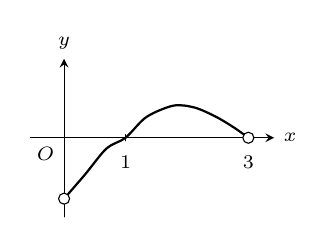
\begin{tikzpicture}[x=.78cm,y=.85cm,>=stealth,line cap=round,line join=round,
  every node/.style={font=\scriptsize}]
  \draw[->] (-.55,0)--(3.42,0) node[right] {$x$};
  \draw[->] (0,-1.18)--(0,1.18) node[above] {$y$};
  \node[below left] at (0,0) {$O$};
  \draw (.0,.045)--(.0,-.045);
  \draw (1,.045)--(1,-.045) node[below=2pt] {$1$};
  \draw (3,.045)--(3,-.045) node[below=2pt] {$3$};
  \draw[thick] plot[smooth] coordinates {
    (0,-.91) (.34,-.55) (.69,-.16) (1,0) (1.34,.31)
    (1.78,.48) (2.13,.45) (2.48,.31) (2.77,.15) (3,0)
  };
  \filldraw[fill=white] (0,-.91) circle[radius=2pt];
  \filldraw[fill=white] (3,0) circle[radius=2pt];
\end{tikzpicture}
\end{center}
\nopagebreak[4]
（A）\(\left(-3,-\dfrac\pi2\right)\cup(0,1)\cup\left(\dfrac\pi2,3\right)\)

（B）\(\left(-\dfrac\pi2,-1\right)\cup(0,1)\cup\left(\dfrac\pi2,3\right)\)

（C）\((-3,-1)\cup(0,1)\cup(1,3)\)　　（D）\(\left(-3,-\dfrac\pi2\right)\cup(0,1)\cup(1,3)\)

\Needspace{0.4\textheight}
\end{question}
\begin{question}
\gkti{12}如图所示，\(f_i(x)\ (i=1,2,3,4)\) 是定义在 \([0,1]\) 上的四个函数，其中满足性质：“对 \([0,1]\) 中任意的 \(x_1\) 和 \(x_2\)，任意 \(\lambda\in[0,1]\)，\(f[\lambda x_1+(1-\lambda)x_2]\leqslant\lambda f(x_1)+(1-\lambda)f(x_2)\) 恒成立”的只有\mbox{（　　）}。
\nopagebreak[4]
\begin{center}% 第 12 题四幅函数图的源图结构重绘；曲线高度与弯曲程度仅示意。
% 虚线 x=1 只出现在 f_2、f_3、f_4 面板，与固定 PDF 第 1 页一致。
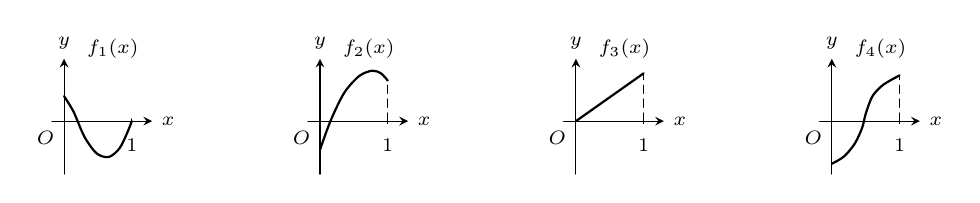
\begin{tikzpicture}[x=.86cm,y=.66cm,>=stealth,line cap=round,line join=round,
  every node/.style={font=\scriptsize}]
\foreach \shift/\name in {0/{f_1(x)},3.25/{f_2(x)},6.50/{f_3(x)},9.75/{f_4(x)}} {
  \begin{scope}[xshift=\shift cm]
    \draw[->] (-.18,0)--(1.30,0) node[right] {$x$};
    \draw[->] (0,-1.02)--(0,1.20) node[above] {$y$};
    \node[below left] at (0,0) {$O$};
    \draw (1,.045)--(1,-.045) node[below=2pt] {$1$};
    \node[above] at (.72,1.02) {$\name$};
  \end{scope}
}
% f_1：先降后升，右端在 x=1 处回到 x 轴；无辅助虚线。
\begin{scope}
  \draw[thick] plot[smooth] coordinates {
    (0,.48) (.14,.18) (.30,-.30) (.48,-.62) (.66,-.69)
    (.82,-.52) (.94,-.20) (1,0)
  };
\end{scope}
% f_2：从负值起始，凹向下上升并在 x=1 处收尾。
\begin{scope}[xshift=3.25cm]
  \draw[thick] plot[smooth] coordinates {
    (0,-.55) (.16,.02) (.36,.55) (.58,.87) (.77,.97) (.90,.92) (1,.78)
  };
  \draw[densely dashed] (1,0)--(1,.78);
\end{scope}
% f_3：从原点出发的线段，右端为 x=1。
\begin{scope}[xshift=6.50cm]
  \draw[thick] (0,0)--(1,.92);
  \draw[densely dashed] (1,0)--(1,.92);
\end{scope}
% f_4：下凸后上凸的 S 形曲线，穿过 x 轴后到达 x=1 端点。
\begin{scope}[xshift=9.75cm]
  \draw[thick] plot[smooth] coordinates {
    (0,-.82) (.18,-.68) (.34,-.43) (.45,-.12) (.50,.14)
    (.60,.48) (.76,.70) (1,.88)
  };
  \draw[densely dashed] (1,0)--(1,.88);
\end{scope}
\end{tikzpicture}
\end{center}
\nopagebreak[4]
（A）\(f_1(x),f_3(x)\)　　（B）\(f_2(x)\)　　（C）\(f_2(x),f_3(x)\)　　（D）\(f_4(x)\)

\end{question}
\gkpart{二、填空题}

\begin{question}
\gkti{13}\(\arcsin\left(-\dfrac25\right),\ \arccos\left(-\dfrac34\right),\ \arctan\left(-\dfrac54\right)\) 从小到大的顺序是\gkblank{}。

\end{question}
\begin{question}
\gkti{14}等差数列 \(\{a_n\}\) 中，\(a_1=2\)，公差不为零，且 \(a_1,a_3,a_{11}\) 恰好是某等比数列的前三项，那么该等比数列公比的值等于\gkblank{}。

\end{question}
\begin{question}
\gkti{15}关于直角 \(AOB\) 在平面 \(\alpha\) 内的射影有如下判断：①可能是 \(0^\circ\) 的角；②可能是锐角；③可能是直角；④可能是直角；⑤可能是 \(180^\circ\) 的角。其中正确的序号是\gkblank{}。（注：把你认为正确判断的序号都填上。）

\begin{gktip}
原件 Q15 中③、④均印作“可能是直角”；此处按固定 PDF 原文照录，未推测或改正。
\end{gktip}

\end{question}
\begin{question}
\gkti{16}已知 \(P\) 是直线 \(3x+4y+8=0\) 上的动点，\(PA,PB\) 是圆 \(x^2+y^2-2x-2y+8=0\) 的两条切线，\(A,B\) 是切点，\(C\) 是圆心，那么四边形 \(PACB\) 面积的最小值为\gkblank{}。

\end{question}
\gkpart{三、解答题}

\begin{question}
\gkti{17}解不等式 \(\left|\sqrt{2x-1}-x\right|<2\)。

\Needspace{0.4\textheight}
\end{question}
\begin{question}
\gkti{18}如图，在多面体 \(ABCD-A_1B_1C_1D_1\) 中，上、下底面平行且均为矩形，相对的侧面与同一底面所成的二面角大小相等，侧棱延长后相交与 \(E,F\) 两点。上、下底面矩形的长、宽分别为 \(c,d\) 与 \(a,b\)，且 \(a>c,b>d\)，两底面间的距离为 \(h\)。

（1） 求侧面 \(ABB_1A_1\) 与底面 \(ABCD\) 所成二面角的大小；

（2） 证明：\(EF\parallel ABCD\)；

\Needspace{5\baselineskip}
（3） 在估侧该多面体的体积时，经常运用近似公式 \(V_{\text{估}}=S_{\text{中截面}}\cdot h\) 来计算，已知它的体积公式是
\nopagebreak[4]
\[
V=\frac{h}{6}\left(S_{\text{上底面}}+4S_{\text{中截面}}+S_{\text{下底面}}\right),
\]
试判断 \(V_{\text{估}}\) 与 \(V\) 的大小关系，并加以证明。

注：与两个底面平行，且到两个底面距离相等的截面称为该多面体的中截面。
\nopagebreak[4]
\begin{center}% 第 18 题多面体源图的拓扑重绘：上下底面为矩形，侧棱延长形成 E、F。
% 所有长度比例仅为示意；尺寸标签 a,b,c,d 保留，图中不增添 h。
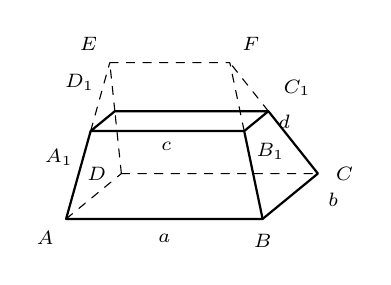
\begin{tikzpicture}[x=.78cm,y=.72cm,line cap=round,line join=round,
  every node/.style={font=\scriptsize}]
  \coordinate (A)  at (0,0);
  \coordinate (B)  at (3.2,0);
  \coordinate (C)  at (4.1,.8);
  \coordinate (D)  at (.9,.8);
  \coordinate (A1) at (.4,1.55);
  \coordinate (B1) at (2.9,1.55);
  \coordinate (C1) at (3.294,1.9);
  \coordinate (D1) at (.794,1.9);
  \coordinate (E)  at (.711,2.756);
  \coordinate (F)  at (2.666,2.756);

  % 可见棱
  \draw[thick] (A)--(B)--(C)--(C1)--(B1)--(A1)--(D1)--(C1);
  \draw[thick] (A)--(A1) (B)--(B1);
  % 隐藏棱
  \draw[dashed] (A)--(D) (D)--(C) (D)--(D1);
  % 侧棱延长线及交点 E、F；与源图一样用虚线表示。
  \draw[dashed] (A1)--(E) (D1)--(E) (B1)--(F) (C1)--(F) (E)--(F);

  % 源图尺寸标签仅标在线段附近，不画尺寸箭头。
  \node at (1.6,-.34) {$a$};
  \node at (4.35,.33) {$b$};
  \node at (1.63,1.28) {$c$};
  \node at (3.55,1.72) {$d$};

  \node[below left=1pt] at (A) {$A$};
  \node[below=2pt] at (B) {$B$};
  \node[right=3pt] at (C) {$C$};
  \node[left=2pt] at (D) {$D$};
  \node[below left=3pt] at (A1) {$A_1$};
  \node[below right=1pt] at (B1) {$B_1$};
  \node[above right=2pt] at (C1) {$C_1$};
  \node[above left=4pt] at (D1) {$D_1$};
  \node[above left=1pt] at (E) {$E$};
  \node[above right=1pt] at (F) {$F$};
\end{tikzpicture}
\end{center}
\nopagebreak[4]
\end{question}
\begin{question}
\gkti{19}数列 \(\{a_n\}\) 由下列条件确定：\(x_1=a>0\)，
\nopagebreak[4]
\[
x_{n+1}=\frac12\left(x_n+\frac{a}{x_n}\right),\quad n\in\mathbb N.
\]

（1） 证明：对 \(n\geqslant2\)，总有 \(x_n\geqslant\sqrt a\)；

（2） 证明：对 \(n\geqslant2\)，总有 \(x_n\geqslant x_{n+1}\)；

（3） 若数列 \(\{a_n\}\) 的极限存在，且大于零，求 \(\lim_{n\to\infty}x_n\) 的值。

\end{question}
\begin{question}
\gkti{20}在研究并行计算的基本算法时，有以下简单模型问题：用计算机求 \(n\) 个不同的数 \(v_1,v_2,\ldots,v_n\) 的和
\nopagebreak[4]
\[
\sum_{i=1}^{n}v_i=v_1+v_2+\cdots+v_n,
\]
计算开始前，\(n\) 个数存贮在 \(n\) 台由网络连接的计算机中，每台机器存一个数。计算开始后，在一个单位时间内，每台机器至多到一台其他机器中读数据，并与自己原有数据相加得到新的数据，各台机器可同时完成上述工作。为了用尽可能少的单位时间，即可完成计算，方法可用下表表示（表中「1 读」「1 果」分别表示第一单位时间的被读机号与结果，其余类推；表头为排印缩写，原页为「第一单位时间·被读机号」等全称）：

\begin{center}
\begingroup\setlength{\tabcolsep}{4pt}
\begin{tabular}{cccccccc}
\toprule
机器号 & 初始 & 1 读 & 1 果 & 2 读 & 2 果 & 3 读 & 3 果 \\
\midrule
1 & \(v_1\) & 2 & \(v_1+v_2\) &  &  &  &  \\
2 & \(v_2\) & 1 & \(v_2+v_1\) &  &  &  &  \\
\bottomrule
\end{tabular}
\endgroup
\end{center}

（1） 当 \(n=4\) 时，至少需要多少个单位时间可完成计算？把你设计的方法填入下表：

\begin{center}
\begingroup\setlength{\tabcolsep}{4pt}
\begin{tabular}{cccccccc}
\toprule
机器号 & 初始 & 1 读 & 1 果 & 2 读 & 2 果 & 3 读 & 3 果 \\
\midrule
1 & \(v_1\) &  &  &  &  &  &  \\
2 & \(v_2\) &  &  &  &  &  &  \\
3 & \(v_3\) &  &  &  &  &  &  \\
4 & \(v_4\) &  &  &  &  &  &  \\
\bottomrule
\end{tabular}
\endgroup
\end{center}

（2） 当 \(n=128\) 时，要使所有机器都得到 \(\displaystyle\sum_{i=1}^{n}v_i\)，至少需要多少个单位时间可完成计算？（结论不要求证明）

\end{question}
\begin{question}
\gkti{21}已知 \(O(0,0),B(1,0),C(b,c)\) 是 \(\triangle OBC\) 的三个顶点。

（1） 写出 \(\triangle OBC\) 的重心 \(G\)、外心 \(F\)、垂心 \(H\) 的坐标，并证明 \(G,F,H\) 三点共线；

（2） 当直线 \(FH\) 与 \(OB\) 平行时，求顶点 \(C\) 的轨迹。

\end{question}
\begin{question}
\gkti{22}已知 \(f(x)\) 是定义在 \(\mathbb R\) 上的不恒为零的函数，且对于任意的 \(a,b\in\mathbb R\) 都满足：
\nopagebreak[4]
\[
f(a\cdot b)=af(b)+bf(a).
\]

（1） 求 \(f(0),f(1)\) 的值；

（2） 判断 \(f(x)\) 的奇偶性，并证明你的结论；

（3） 若 \(f(2)=2\)，\(u_n=\dfrac{f(2^{-n})}{n}\ (n\in\mathbb N)\)，求数列 \(\{u_n\}\) 的前 \(n\) 项的和 \(S_n\)。

\end{question}